% !TeX root = ../seminar.tex
\section{Roman and Rubin}

{\setbeamercolor{background canvas}{bg=black}
\begin{frame}[plain]
\begin{tikzpicture}[remember picture, overlay]
  \node[inner sep=0] at (current page.center) {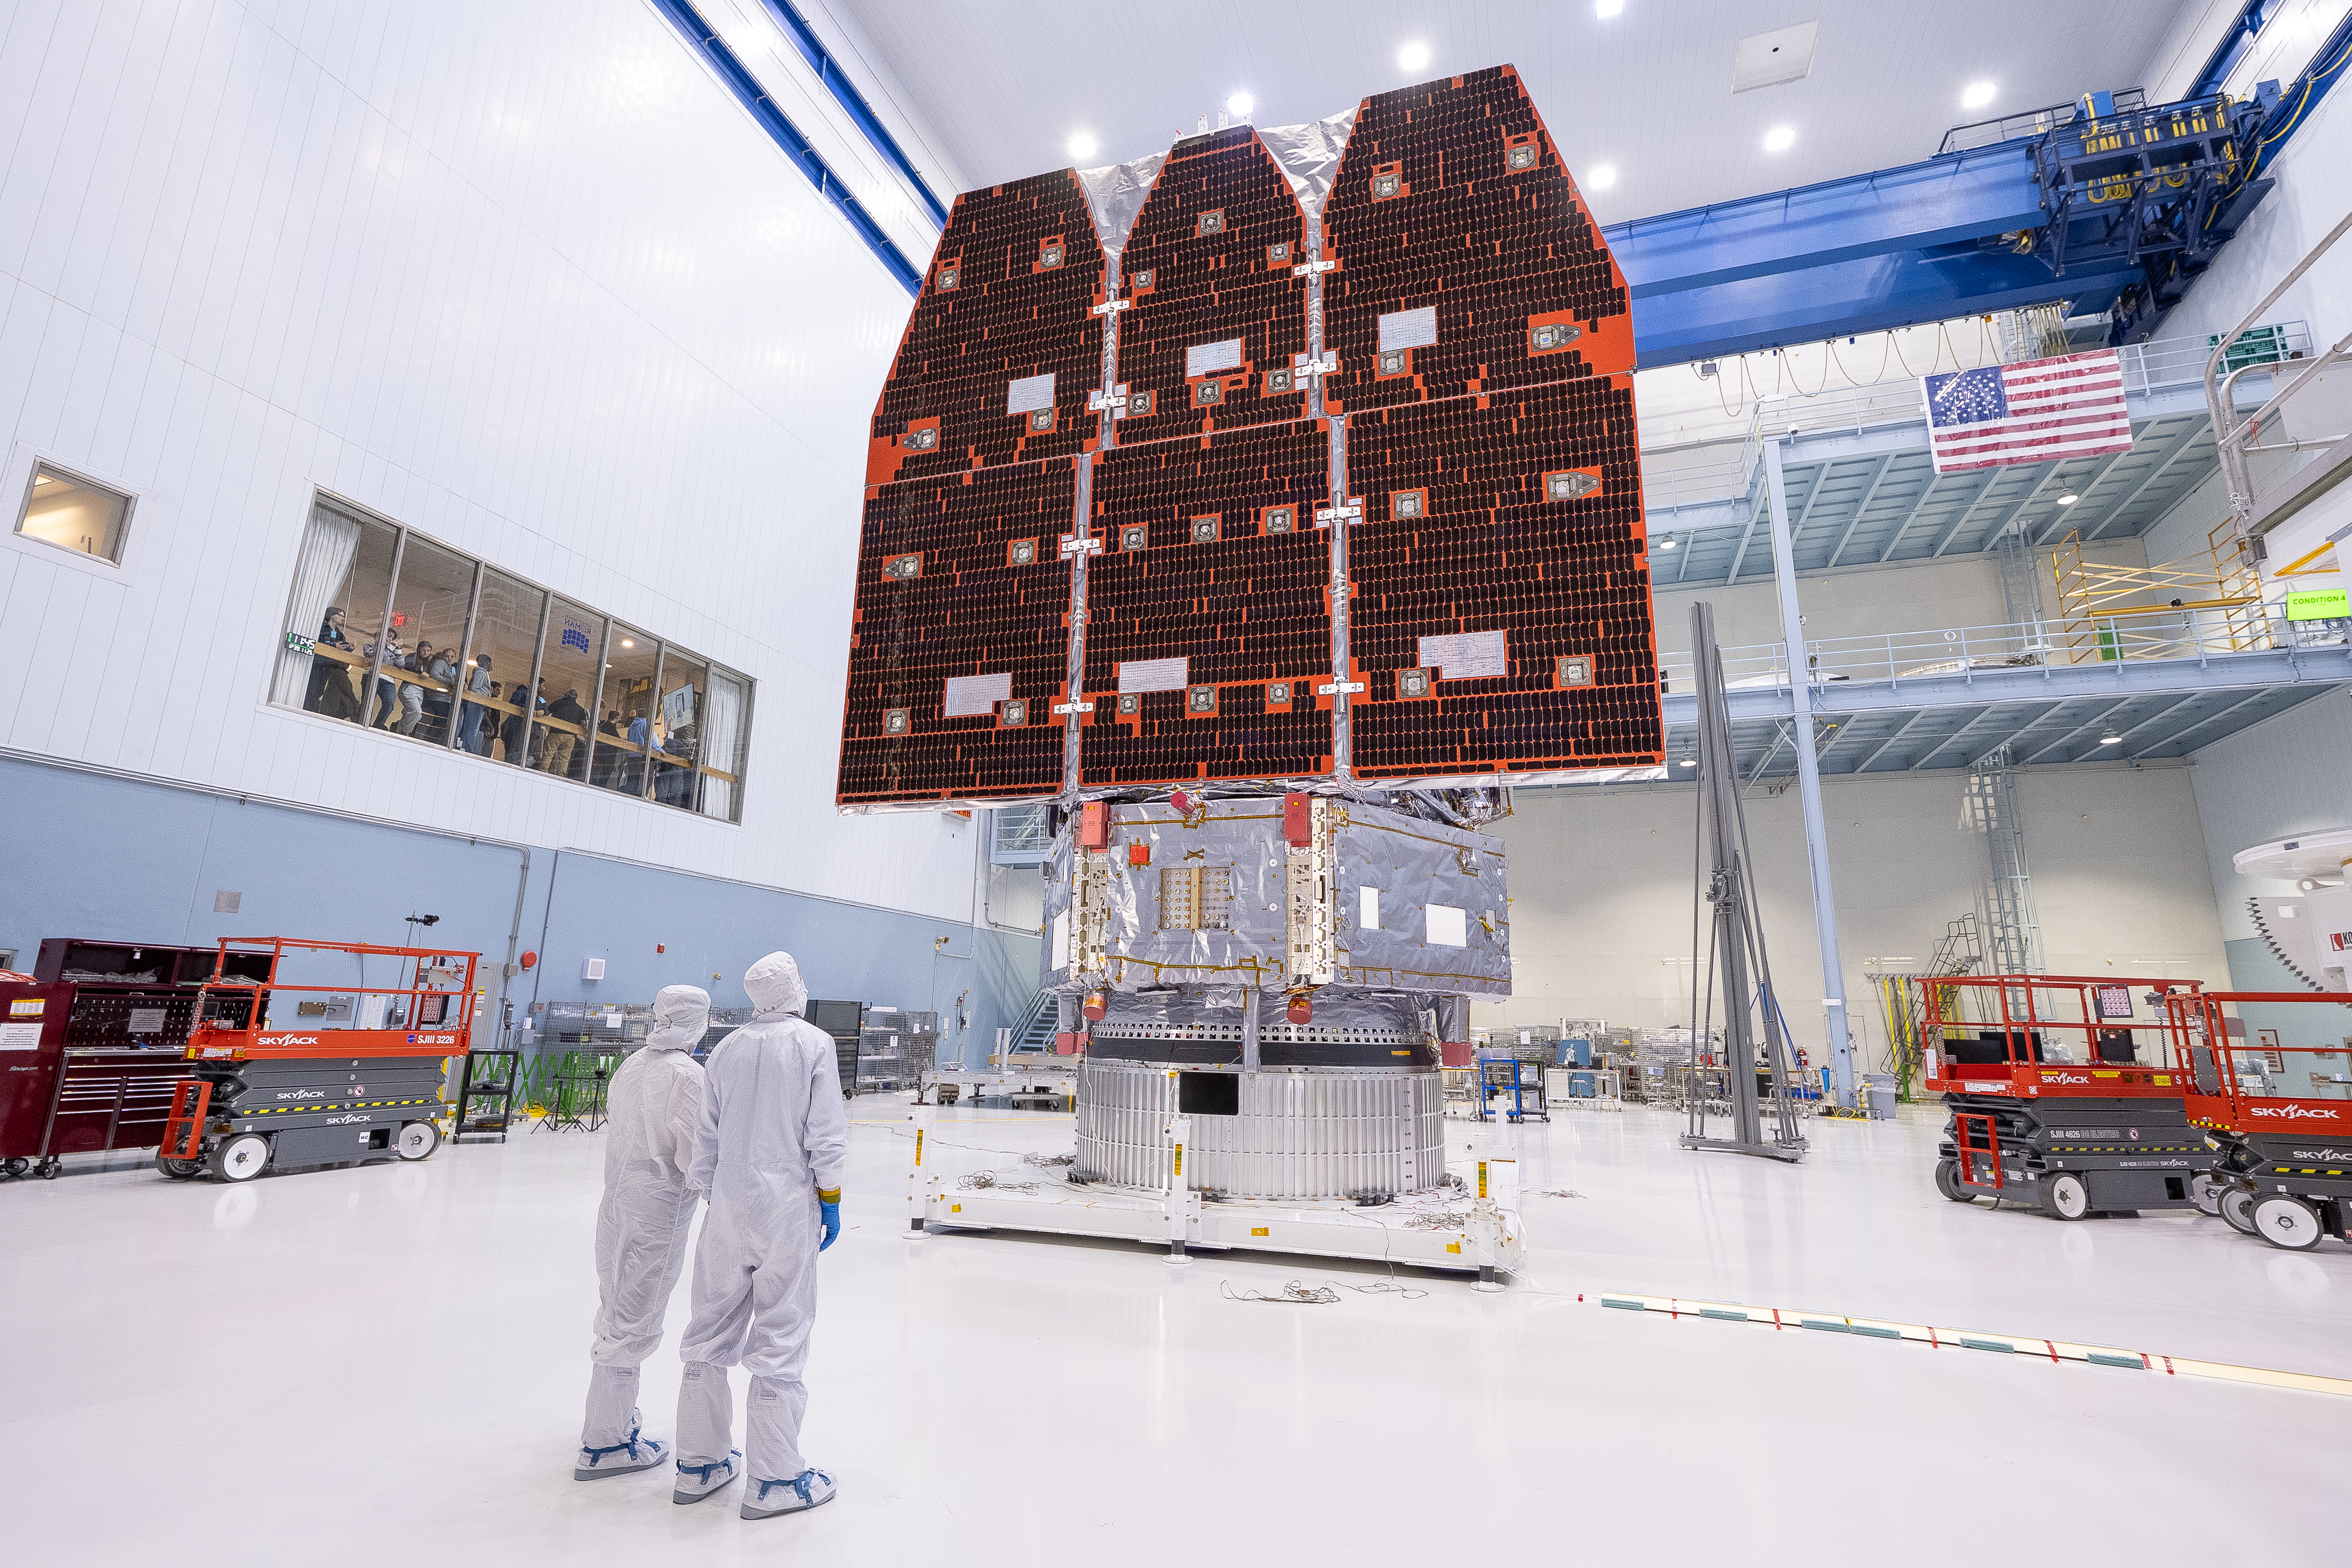
\includegraphics[width=\paperwidth]{roman_assembled}};
  \node[bleedtitle, anchor=north west] at ([xshift=5mm, yshift=-4mm]current page.north west)
       {Roman, fully assembled};
  \node[bleedtext, anchor=north west] at ([xshift=5mm, yshift=-15mm]current page.north west)
       {A $2.4$\,m mirror like \emph{Hubble}'s,\\ a field of view $\sim\!100\times$ larger};
  \bleedcredit{\href{https://www.nasa.gov/image-article/nasas-nancy-grace-roman-space-telescope-completed/}{NASA/Jolearra Tshiteya}}
  \bleedsection
\end{tikzpicture}
\note{\begin{itemize}
  \item NASA Goddard clean room, November 2025: the telescope and spacecraft joined. The technicians give the scale.
  \item Wide Field Instrument: $0.28$\,deg$^2$ per pointing, near-infrared, diffraction-limited.
\end{itemize}}
\end{frame}}


\begin{frame}{Roman's Galactic Bulge Time Domain Survey}
\vspace{2mm}
\begin{columns}[c]
\begin{column}{.56\linewidth}
\centering
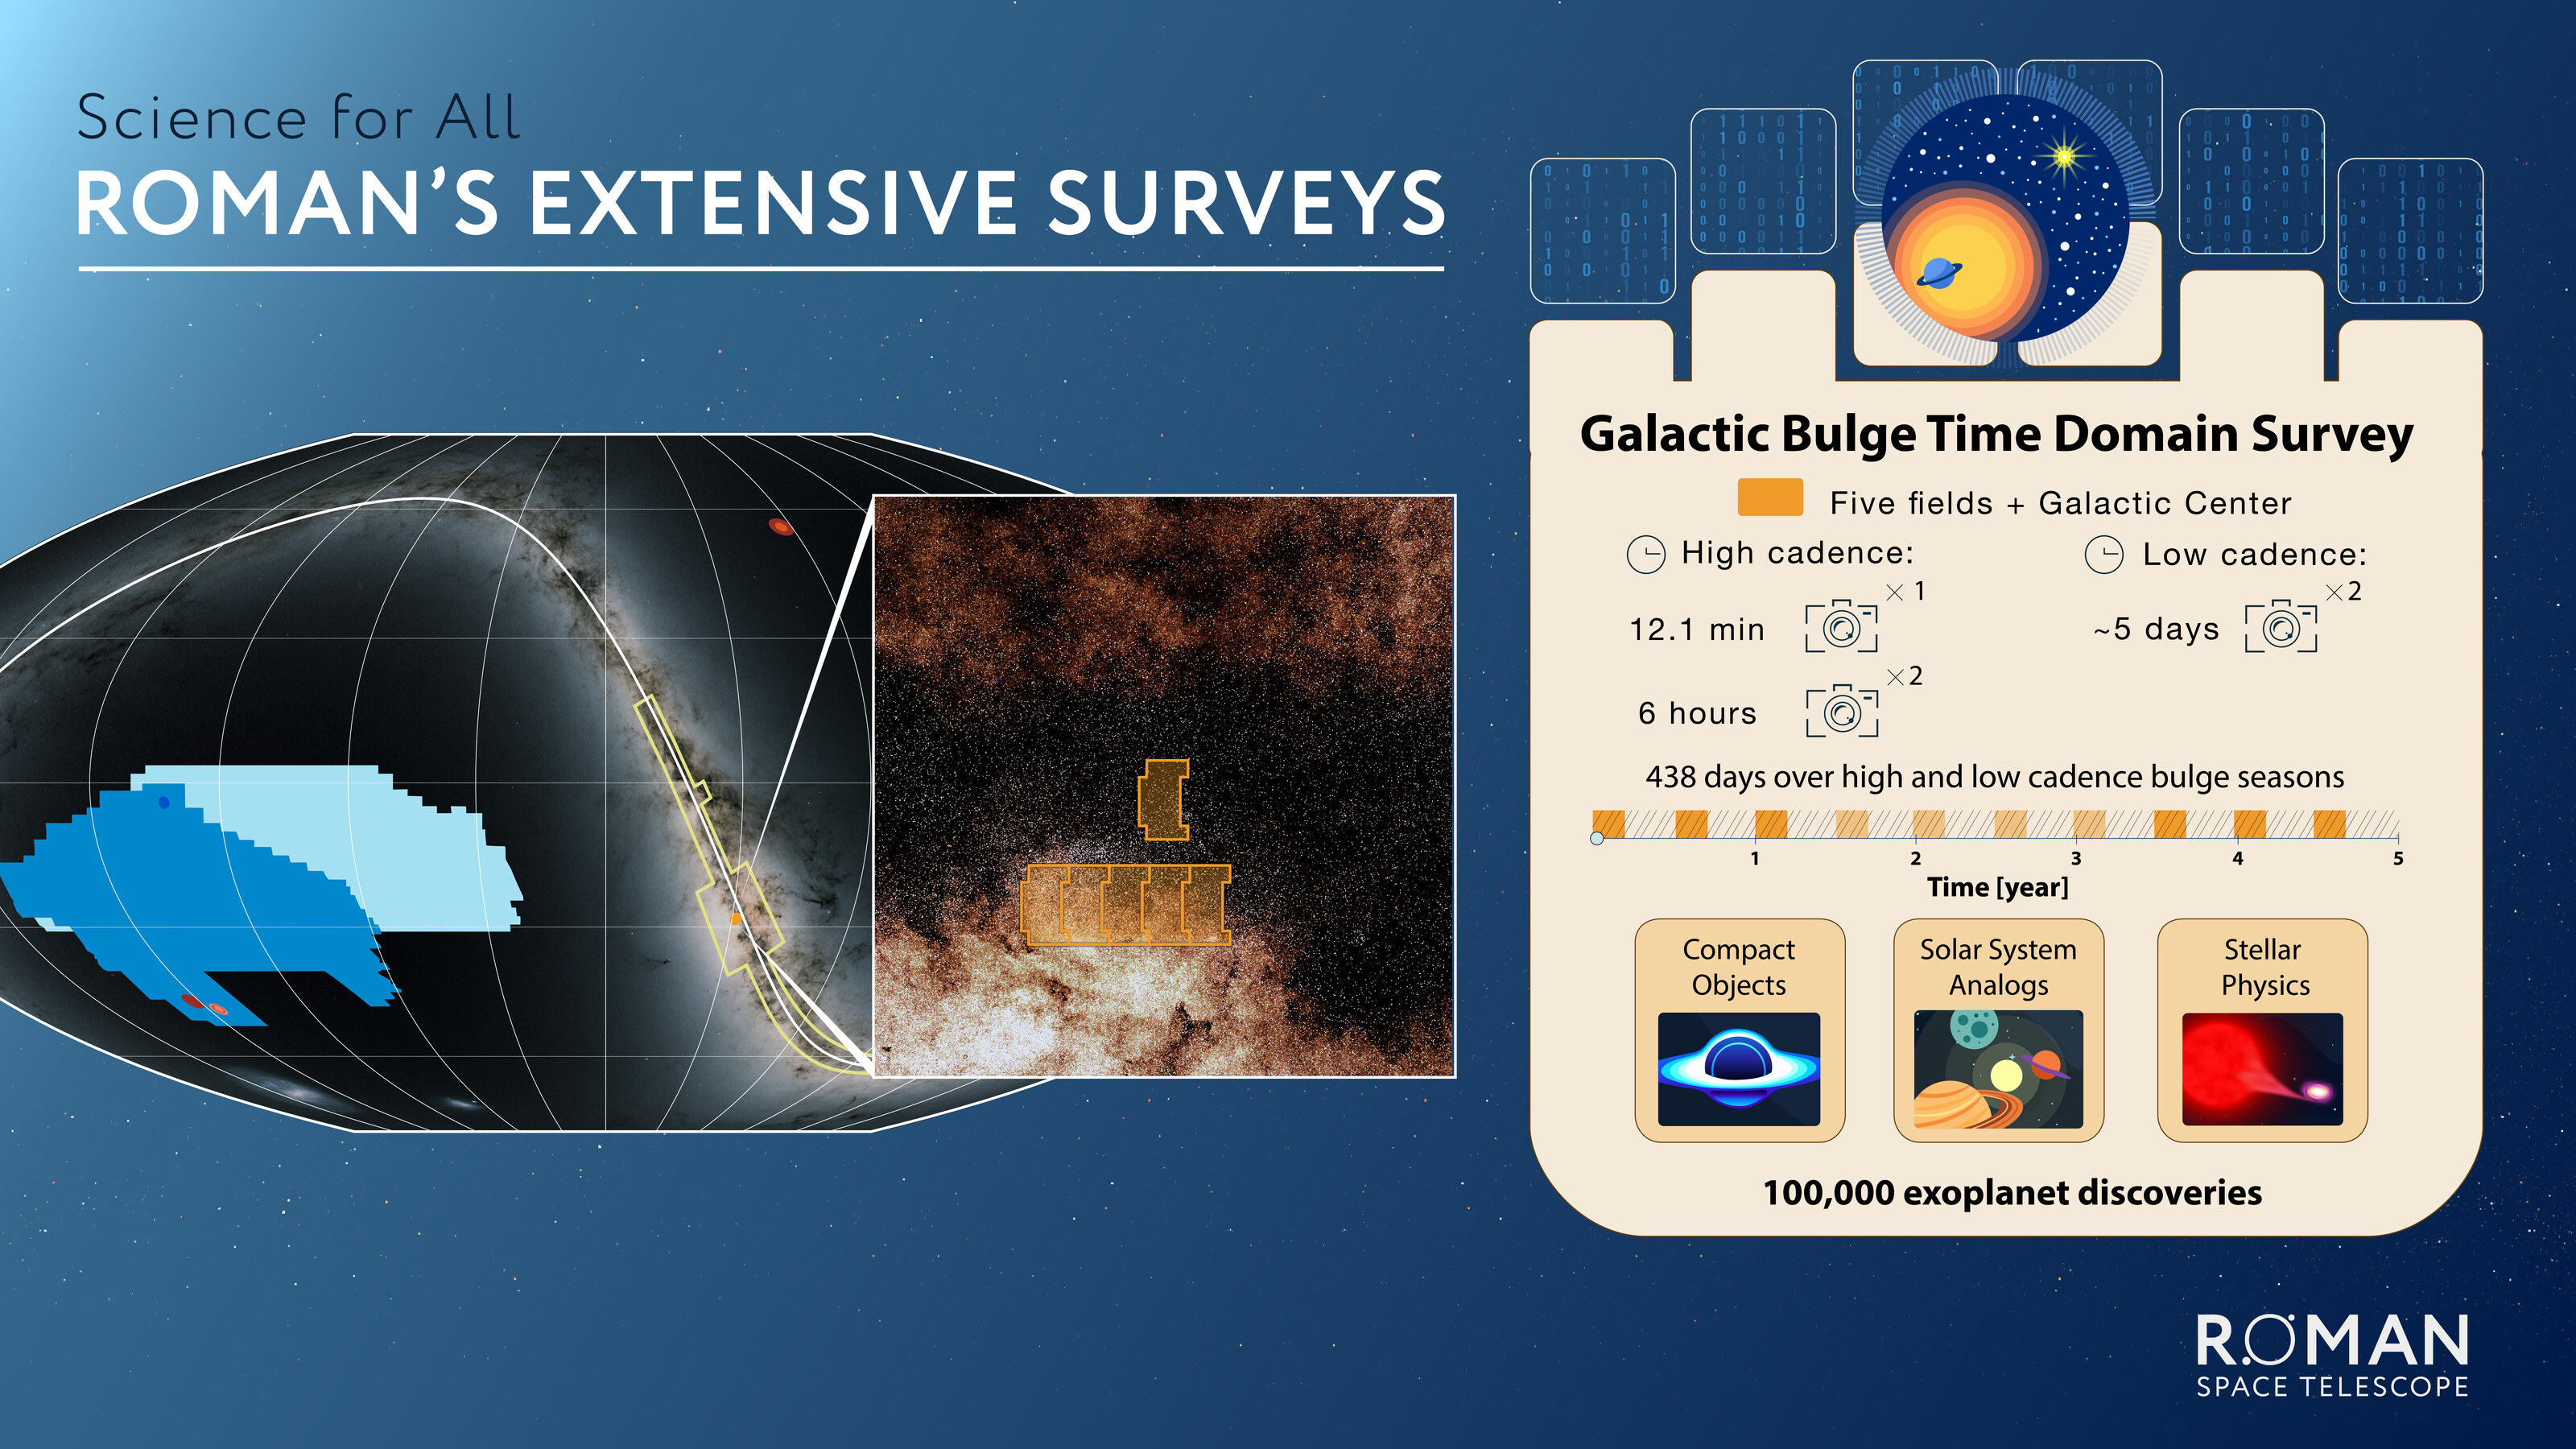
\includegraphics[width=.95\linewidth]{roman_gbtds_infographic}\\[2mm]
\credit{\href{https://roman-docs.stsci.edu/roman-community-defined-surveys/galactic-bulge-time-domain-survey}{STScI, Roman Galactic Bulge Time Domain Survey}}
\end{column}
\begin{column}{.40\linewidth}
\begin{itemize}\setlength{\itemsep}{5pt}
  \item<+-> Six fields, $1.7$\,deg$^2$
  \item<+-> Near-infrared: \textbf{little dust}
  \item<+-> An exposure every $12$\,min
  \item<+-> $\sim\!1$\,mas \textbf{astrometry}
  \item<+-> At \textbf{L2}: a second viewpoint\\ for the parallax?
\end{itemize}
\end{column}
\end{columns}
\vfill
\refnote{\ads{2019ApJS..241....3P}{Penny et al.\ 2019, ApJS 241, 3};
\ads{2019JATIS...5d4005S}{Sanderson et al.\ 2019, JATIS 5, 044005}}
\note{\begin{itemize}
  \item F146 filter: $A_{\rm F146}\approx0.20\,A_V$.
  \item Ten $\sim70$-day seasons: six at high cadence ($12.1$\,min), four at low cadence ($\sim5$\,d); gaps while the
        bulge is near the Sun. $\sim5\times10^4$ exposures per field.
  \item Diffraction-limited: $\sim1$\,mas per exposure for bright stars.
  \item L2 and Earth are $0.01$\,AU apart: a satellite parallax with Rubin was expected to help; the preliminary results test it.
\end{itemize}}
\end{frame}

{\setbeamercolor{background canvas}{bg=black}
\begin{frame}[plain]
\begin{tikzpicture}[remember picture, overlay]
  % portrait photo, full width, cropped to the band of sky and the dome (from 30% of its height down)
  \node[anchor=north, inner sep=0] at ([yshift=7.2cm]current page.north)
       {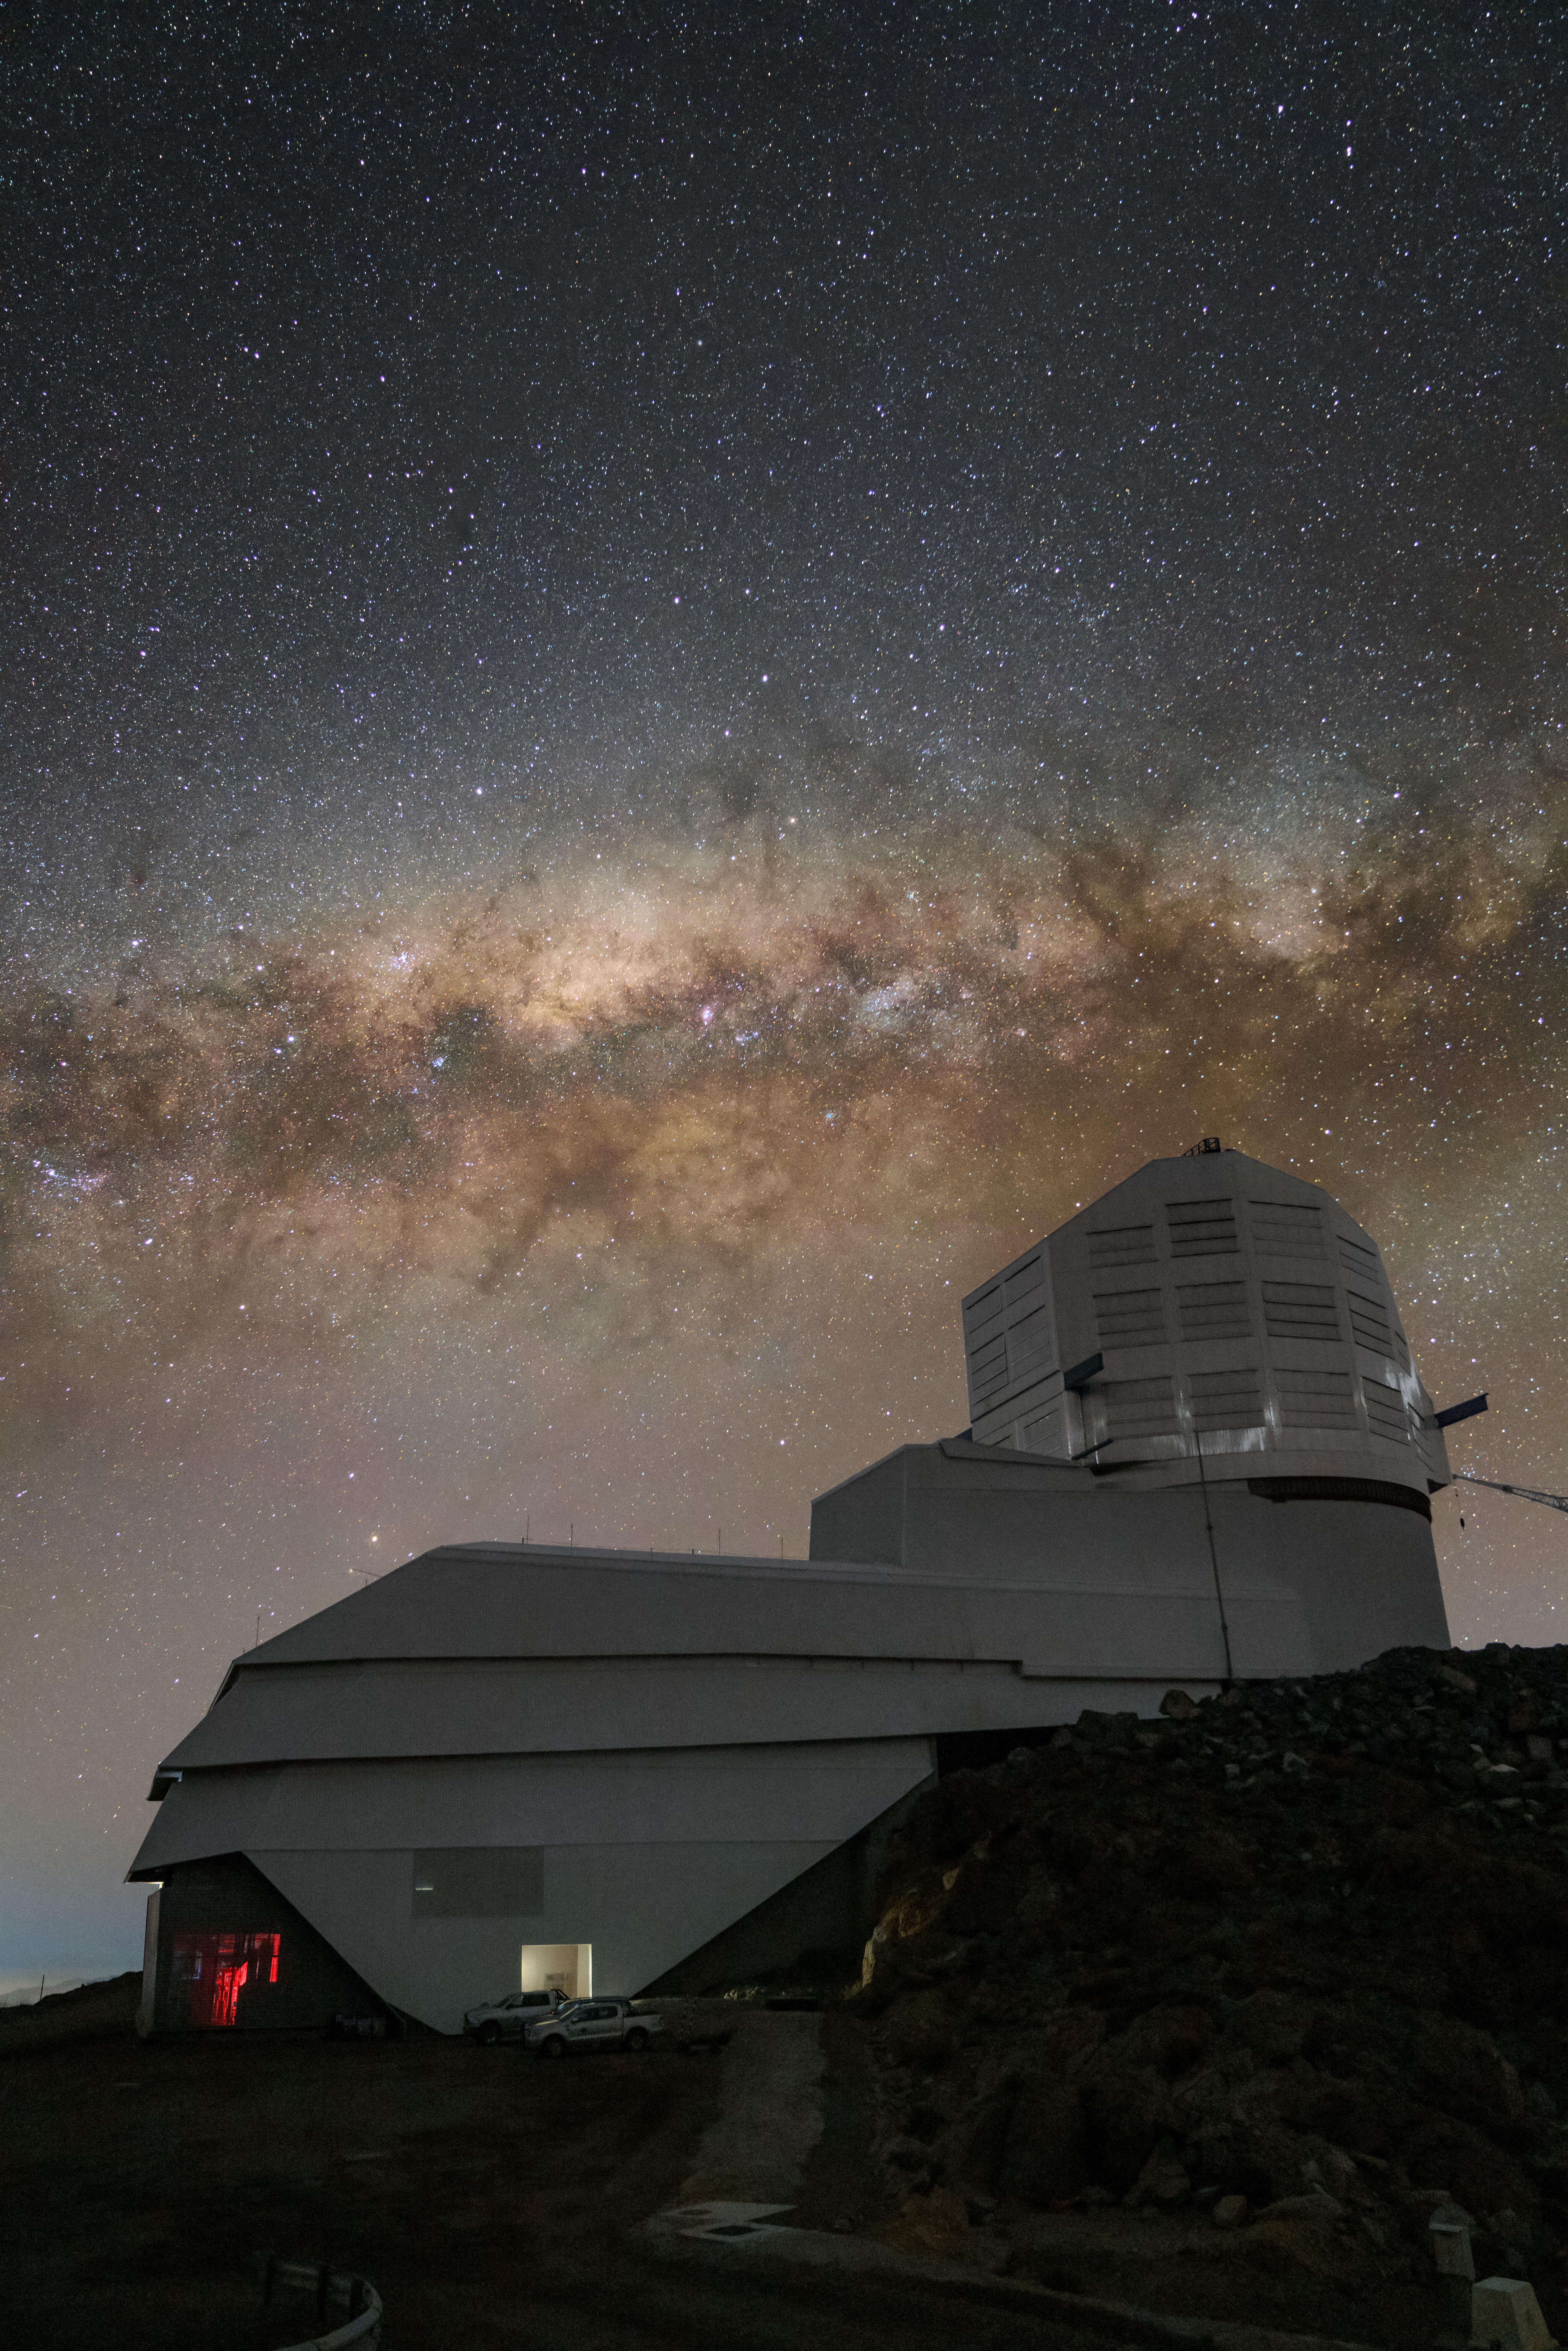
\includegraphics[width=\paperwidth]{rubin_milky_way}};
  \node[bleedtitle, anchor=north west] at ([xshift=5mm, yshift=-4mm]current page.north west)
       {Vera C.\ Rubin Observatory, Chile};
  \node[bleedtext, anchor=north west] at ([xshift=5mm, yshift=-15mm]current page.north west)
       {$8.4$\,m mirror, a $9.6$\,deg$^2$ camera:\\ the whole southern sky every few nights};
  \bleedcredit{\href{https://noirlab.edu/public/images/20220408PachonFPano35mmRubinAux_MW_EQ-001-CC-c3/}{RubinObs/NOIRLab/SLAC/NSF/DOE/AURA/P.~Hor\'alek}}
\end{tikzpicture}
\note{\begin{itemize}
  \item The Galactic bulge rising over Rubin on Cerro Pach\'on.
  \item The Legacy Survey of Space and Time: ten years, optical $ugrizy$, a 3.2-gigapixel camera.
\end{itemize}}
\end{frame}}

\begin{frame}{Rubin, and why the two complement each other}
\vspace{1mm}
\begin{columns}[c]
\begin{column}{.40\linewidth}
\centering
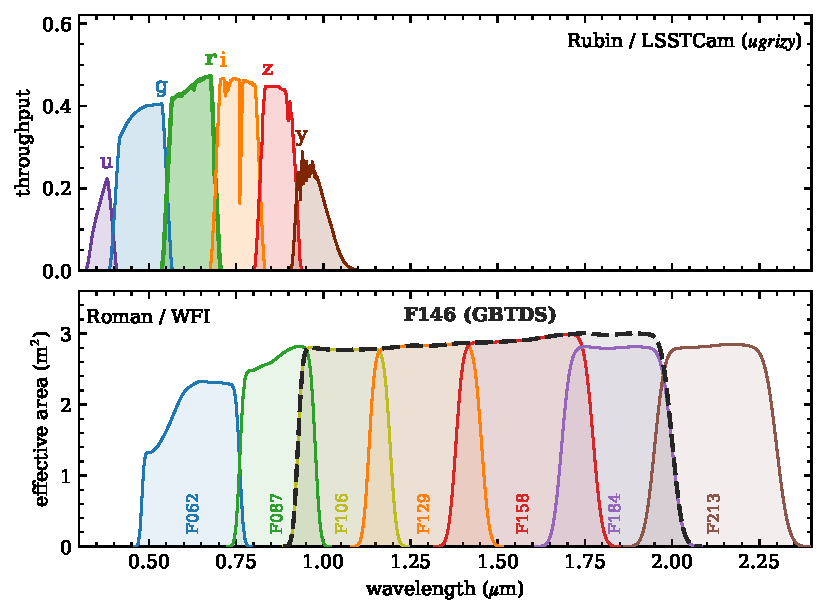
\includegraphics[width=.92\linewidth]{filters}\\[1mm]
\credit{filter curves: \href{http://svo2.cab.inta-csic.es/theory/fps/}{SVO Filter Profile Service}}
\end{column}
\begin{column}{.56\linewidth}
\centering
\textbf{Rubin LSST}: ten years, $ugrizy$, wide sky\\[3mm]
\uncover<2->{%
\renewcommand{\arraystretch}{1.15}
\begin{tabular}{@{}lcc@{}}
\toprule
 & \textbf{Roman} & \textbf{Rubin} \\
\midrule
area & small & large \\
cadence & minutes & days \\
time span & seasons & 10 years \\
dust & mild & severe \\
astrometry & $\sim$1 mas & $\gtrsim$10 mas \\
\bottomrule
\end{tabular}}
\end{column}
\end{columns}
\vspace{4mm}
\uncover<3->{%
\centering
\resizebox{.72\linewidth}{!}{% GENERATED by Report/overview/make_timeline.py -- do not edit.
% sightline (l,b) = (0.40, -1.45); Rubin 2387 epochs, Roman 50401 epochs.
\def\tlL{0.4}\def\tlB{-1.4}\def\tlNrub{2{,}387}\def\tlNrom{50{,}401}
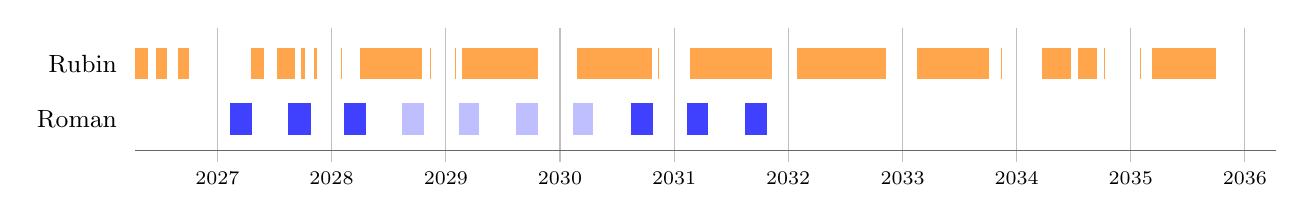
\begin{tikzpicture}[x=1cm,y=1cm]
\draw[black!25] (1.052,-0.15) -- (1.052,1.55);\node[font=\scriptsize,anchor=north] at (1.052,-0.15) {2027};
\draw[black!25] (2.501,-0.15) -- (2.501,1.55);\node[font=\scriptsize,anchor=north] at (2.501,-0.15) {2028};
\draw[black!25] (3.954,-0.15) -- (3.954,1.55);\node[font=\scriptsize,anchor=north] at (3.954,-0.15) {2029};
\draw[black!25] (5.403,-0.15) -- (5.403,1.55);\node[font=\scriptsize,anchor=north] at (5.403,-0.15) {2030};
\draw[black!25] (6.852,-0.15) -- (6.852,1.55);\node[font=\scriptsize,anchor=north] at (6.852,-0.15) {2031};
\draw[black!25] (8.301,-0.15) -- (8.301,1.55);\node[font=\scriptsize,anchor=north] at (8.301,-0.15) {2032};
\draw[black!25] (9.754,-0.15) -- (9.754,1.55);\node[font=\scriptsize,anchor=north] at (9.754,-0.15) {2033};
\draw[black!25] (11.203,-0.15) -- (11.203,1.55);\node[font=\scriptsize,anchor=north] at (11.203,-0.15) {2034};
\draw[black!25] (12.652,-0.15) -- (12.652,1.55);\node[font=\scriptsize,anchor=north] at (12.652,-0.15) {2035};
\draw[black!25] (14.101,-0.15) -- (14.101,1.55);\node[font=\scriptsize,anchor=north] at (14.101,-0.15) {2036};
\draw[black!60] (0,0) -- (14.5,0);
\node[font=\small,anchor=east] at (-0.1,1.1) {Rubin};
\node[font=\small,anchor=east] at (-0.1,0.4) {Roman};
\fill[orange!70] (0.000,0.9) rectangle (0.167,1.3);
\fill[orange!70] (0.270,0.9) rectangle (0.408,1.3);
\fill[orange!70] (0.555,0.9) rectangle (0.686,1.3);
\fill[orange!70] (1.481,0.9) rectangle (1.644,1.3);
\fill[orange!70] (1.809,0.9) rectangle (2.036,1.3);
\fill[orange!70] (2.119,0.9) rectangle (2.170,1.3);
\fill[orange!70] (2.285,0.9) rectangle (2.317,1.3);
\fill[orange!70] (2.620,0.9) rectangle (2.628,1.3);
\fill[orange!70] (2.858,0.9) rectangle (3.647,1.3);
\fill[orange!70] (3.746,0.9) rectangle (3.754,1.3);
\fill[orange!70] (4.065,0.9) rectangle (4.073,1.3);
\fill[orange!70] (4.153,0.9) rectangle (5.128,1.3);
\fill[orange!70] (5.614,0.9) rectangle (6.569,1.3);
\fill[orange!70] (6.652,0.9) rectangle (6.660,1.3);
\fill[orange!70] (7.051,0.9) rectangle (8.098,1.3);
\fill[orange!70] (8.417,0.9) rectangle (9.543,1.3);
\fill[orange!70] (9.941,0.9) rectangle (10.849,1.3);
\fill[orange!70] (11.004,0.9) rectangle (11.011,1.3);
\fill[orange!70] (11.529,0.9) rectangle (11.897,1.3);
\fill[orange!70] (11.981,0.9) rectangle (12.219,1.3);
\fill[orange!70] (12.314,0.9) rectangle (12.322,1.3);
\fill[orange!70] (12.768,0.9) rectangle (12.776,1.3);
\fill[orange!70] (12.926,0.9) rectangle (13.731,1.3);
\fill[blue!75] (1.215,0.2) rectangle (1.489,0.6);
\fill[blue!75] (1.949,0.2) rectangle (2.235,0.6);
\fill[blue!75] (2.665,0.2) rectangle (2.939,0.6);
\fill[blue!25] (3.399,0.2) rectangle (3.677,0.6);
\fill[blue!25] (4.115,0.2) rectangle (4.373,0.6);
\fill[blue!25] (4.849,0.2) rectangle (5.127,0.6);
\fill[blue!25] (5.565,0.2) rectangle (5.823,0.6);
\fill[blue!75] (6.299,0.2) rectangle (6.585,0.6);
\fill[blue!75] (7.015,0.2) rectangle (7.289,0.6);
\fill[blue!75] (7.749,0.2) rectangle (8.035,0.6);
\end{tikzpicture}
}\\[1mm]
\refnote{One sightline in Roman's fields: Rubin's visits (orange), Roman's seasons (blue; dark = high cadence).
\quad Rubin: \ads{2019ApJ...873..111I}{Ivezi\'c et al.\ 2019, ApJ 873, 111}}}
\note{\begin{itemize}
  \item Rubin: $9.6$\,deg$^2$ field of view, from the ground; $\sim2{,}400$ visits per bulge sightline, every few days
        while the bulge is up.
  \item Seeing-limited: $\gtrsim10$\,mas astrometry per visit.
  \item Optical bands are heavily extincted toward the bulge: $A_r\approx0.85\,A_V$ against $0.20\,A_V$ for F146.
\end{itemize}}
\end{frame}

\begin{frame}{What has been forecast so far}
\vspace{2mm}
\begin{columns}[T]
\begin{column}{.32\linewidth}
\centering
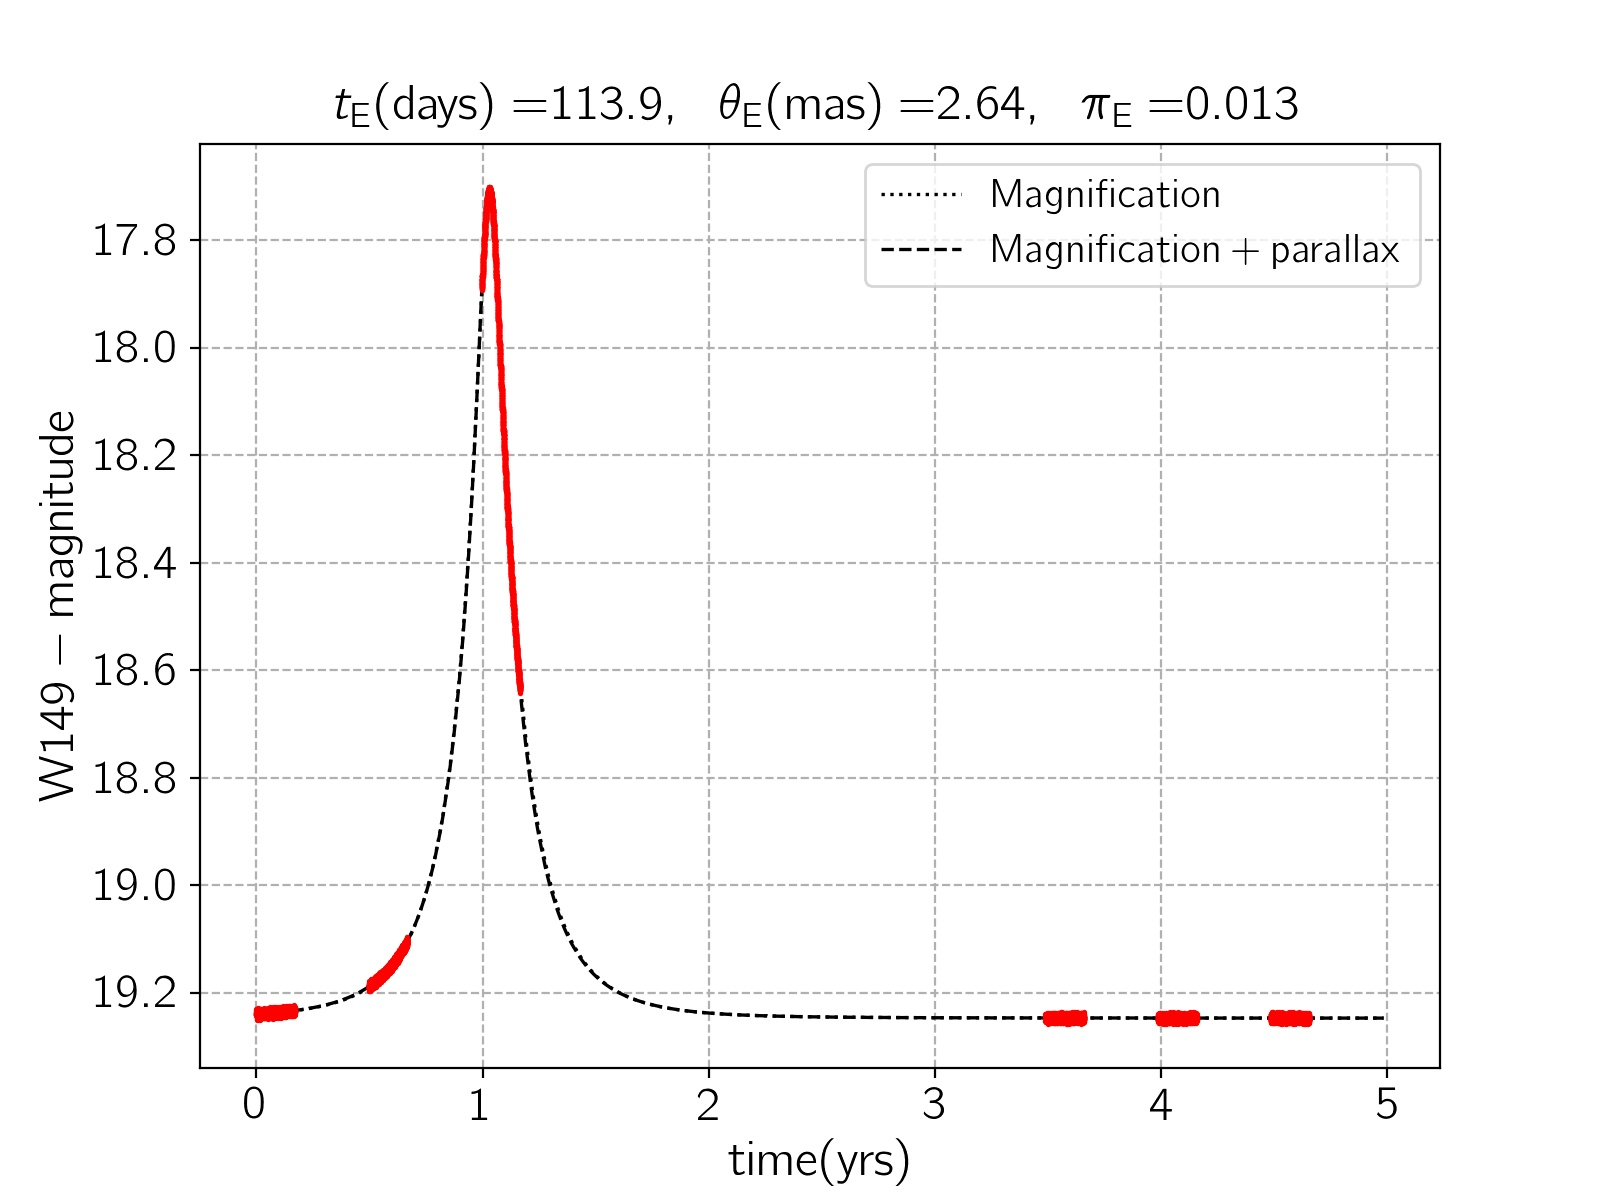
\includegraphics[height=3.2cm]{ss23_lightcurve}\\[1mm]
\credit{\ads{2023AJ....165...96S}{Sajadian \& Sahu 2023}}\\[3mm]
\textbf{Roman}: black-hole masses
\end{column}
\begin{column}{.32\linewidth}
\centering
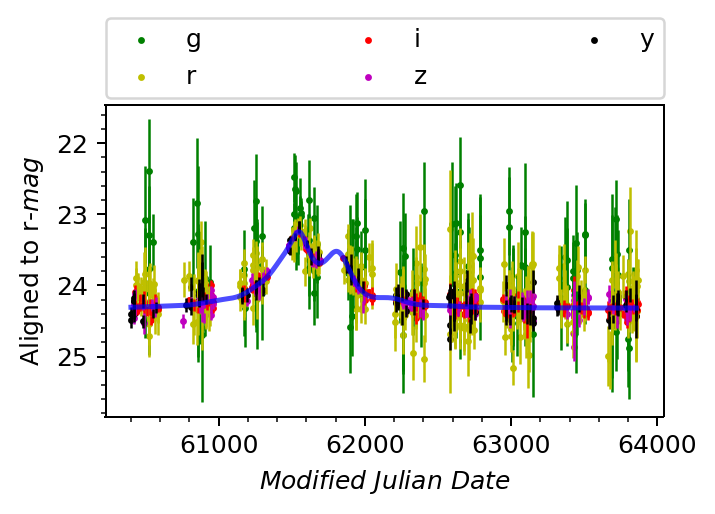
\includegraphics[height=3.2cm]{abrams2025_example}\\[1mm]
\credit{\ads{2025ApJS..276...10A}{Abrams et al.\ 2025}}\\[3mm]
\textbf{Rubin}: characterising events
\end{column}
\begin{column}{.32\linewidth}
\centering
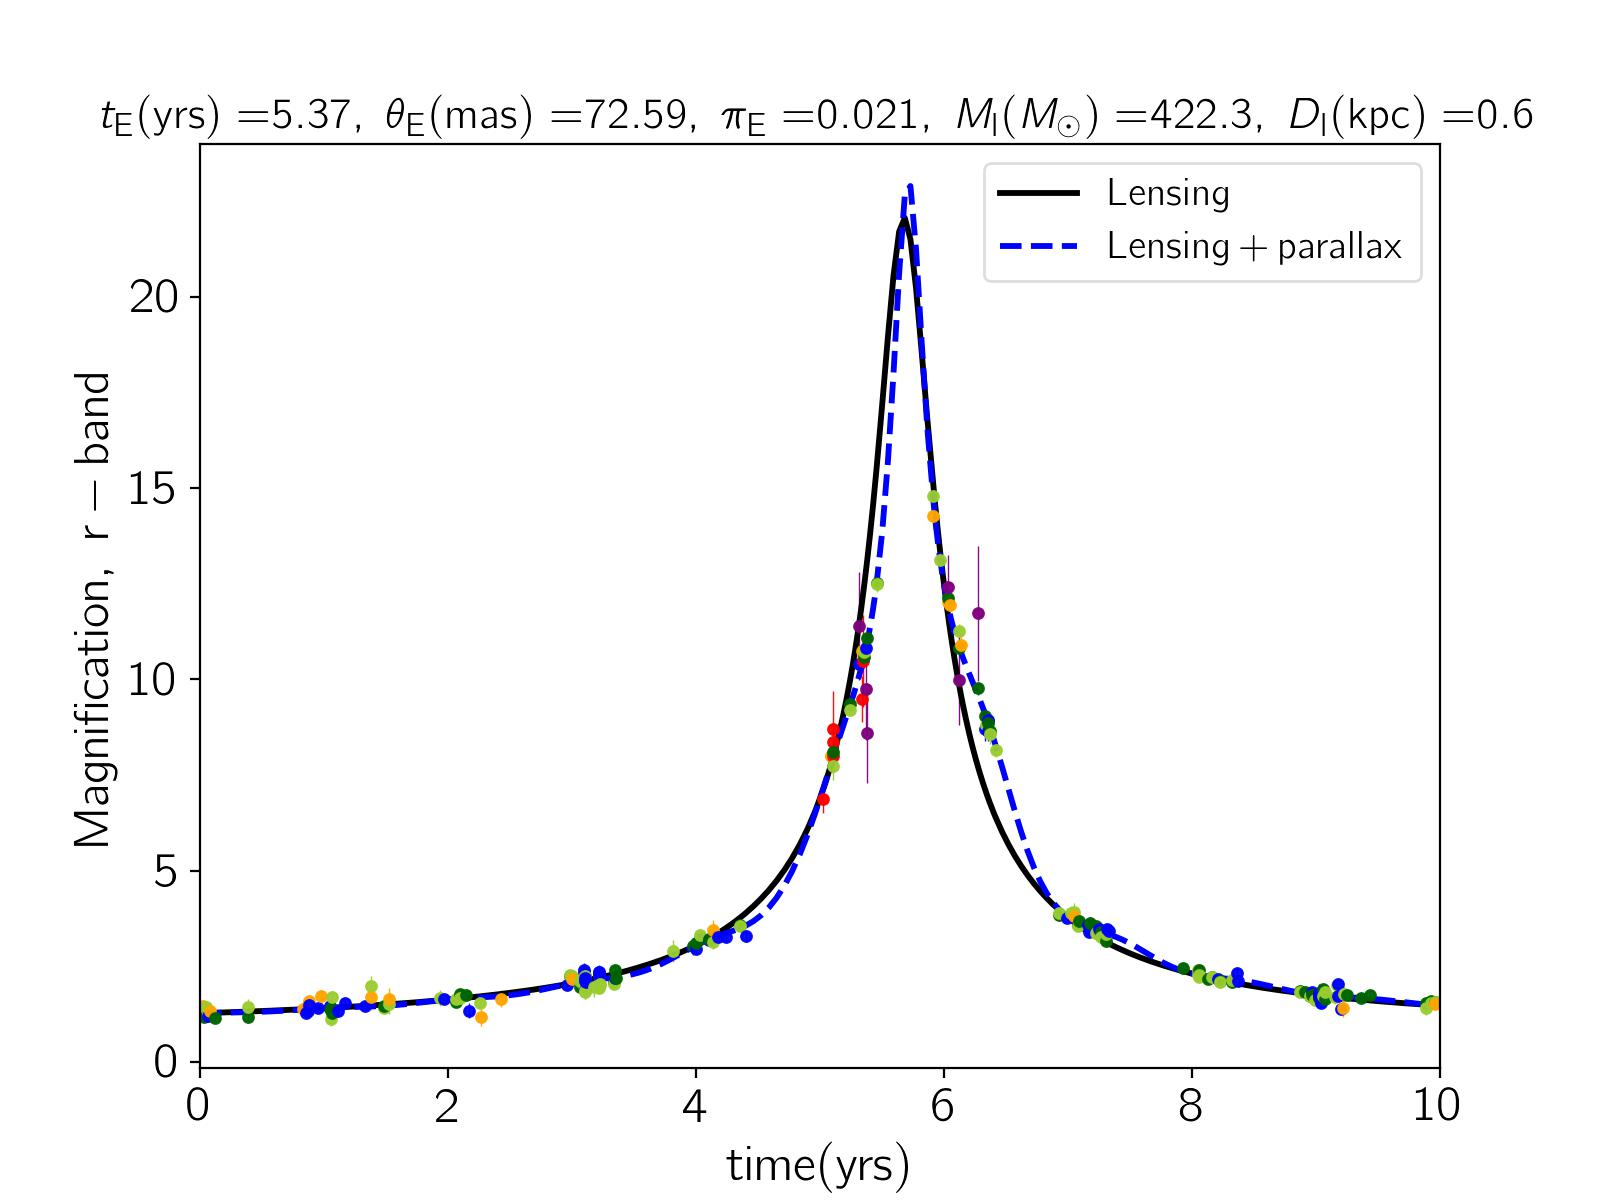
\includegraphics[height=3.2cm]{sm26_lightcurve}\\[1mm]
\credit{\ads{2026ApJ..1009..116S}{Sajadian \& Makler 2026}}\\[3mm]
\textbf{Rubin}: black holes, two images
\end{column}
\end{columns}
\vspace{6mm}
\uncover<2->{%
\begin{beamercolorbox}[rounded=true,sep=6pt,wd=\linewidth]{block body alerted}
\centering
Each telescope alone. \textbf{This thesis: both, on the same events.}
\end{beamercolorbox}}
\note{\begin{itemize}
  \item Sajadian \& Sahu 2023 (AJ 165, 96): Roman alone, isolated black holes; photometric + astrometric Fisher
        forecasts. For $dN/dM\propto M^{-1}$: $\tetE$ to 10\% for $\sim99\%$, the mass for $\sim30\%$ of detections.
  \item Abrams et al.\ 2025 (ApJS 276, 10): which LSST strategies characterise events ($\tE$ and $\piE$) across the
        Galactic plane.
  \item Sajadian \& Makler 2026 (ApJ 1009, 116): Rubin, black holes toward the Magellanic Clouds; images resolvable for
        1.4\% (LMC) and 16.3\% (SMC) of black-hole events.
  \item The thesis: who detects what, what each adds to the other, how many black-hole masses the combination gives.
\end{itemize}}
\end{frame}
